\chapter{Introduction}
\section{Motivation}
In Nature, coloring mostly comes from the inherent colors of materials but sometimes colorization has a pure physical origin such as the effect diffraction or interference of light. Both phenomenon are causing the so called structural coloration, which is the production of color through the interaction of visible light with micrioscopically structured surfaces. 
Color production is die to wave interference with quasiperiodic structures whose periodicity leads to interaction with visible light. Therefore we perceive color when the different wavelengths composing white light are selectively interfered with by matter (absorbed, reflected, refracted, scattered, or diffracted) on their way to our eyes, or when a non-white distribution of light has been emitted.
In animals, such as feathers of birds and the scales of butterflies, interference is created by a range of photonic mechanisms, including diffraction grating, selective mirrors, photonic crystals.
The connection beween microscopic structures and coloration has been observed by Robert Hooke in the early seventeenth centrury. The discovery of the wave nature of light led to the conclusion that the cause for the coloration lies in wave interference.

In the field of computer graphics, many researchers have been attempted rendering of structural colors by formulating a the bidirectional reflectance distribution function (BRDF) for this purpose. But most of the techniques so far, however, are either too slow for interactive rendering or rely on simplifying assumption, like modeling light as rays, to achieve real-time performance, which are not able capturing the essence of diffraction at all. 

\begin{figure}[H]
  \centering
  \subfigure[Elaphe Guttata Snake]{
    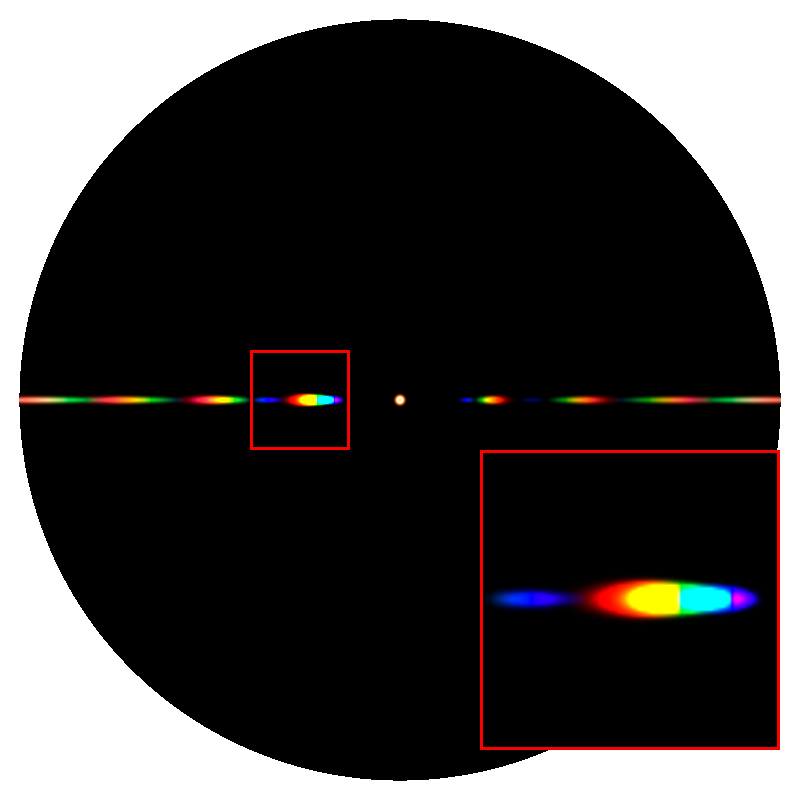
\includegraphics[scale=0.1]{ElapheGuttata/1.png}
    \label{fig:elpahespecies}
  }
~
  \subfigure[Xenopeltis Snake]{
    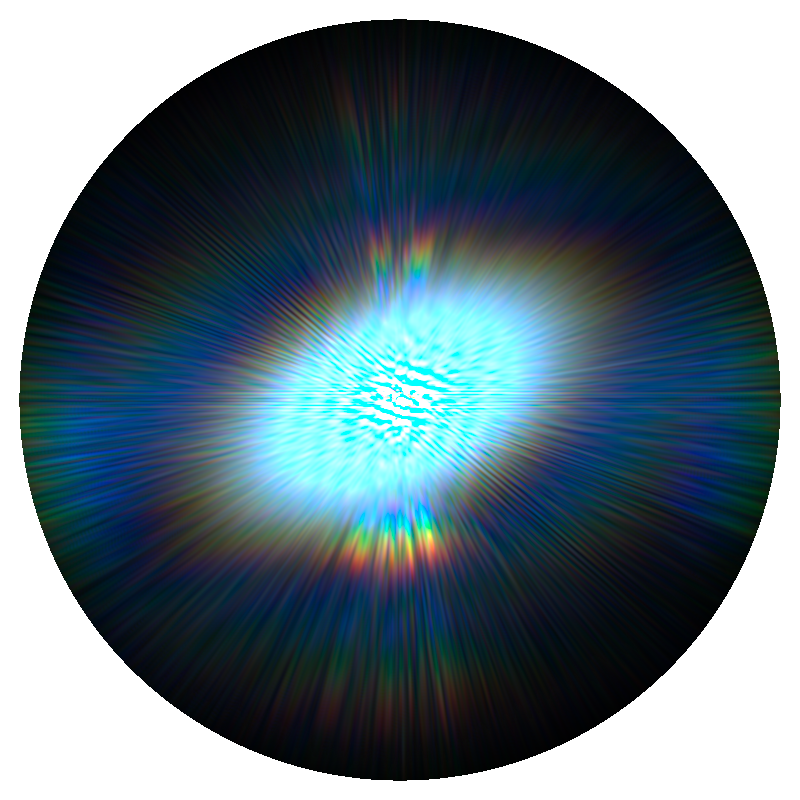
\includegraphics[scale=0.37]{XenopeltisUnicolor/3.png}
    \label{fig:xenospeicies}
  }
  \caption{Effect of diffraction on snake sheds for different species}
  \label{fig:snakespecies}
\end{figure}

\section{Goals}
The purpose of this thesis is to simulate realistically by rendering structural colors caused by the effect of diffraction on different biological structures in realtime. We focus on structural colors generated by diffraction gratings, in particular our approach applies to surfaces with quasiperiodic structures at the nanometer scale that can be represented as heighfields. such structures are found on the sehds of snkaes, wings of butterflies or the bodies of various insects. we restrict ourself and focus on different snake skins sheds which are acquired nanoscaled heightfields using atomic force microscopy. 

In oder to achieve our rendering purpose we will rely J. Stam's formulation of a BRDF which basically describes the effect of diffraction on a given surface assuming one knows the hightfield of this surface and will further extend this. Appart from Stam's approach, which models the heightfield as a probabilistic superposition of bumps and proceeds to derive an analytical expression for the BRDF, our BRDF representation takes the heightfield from explicit measurement. 
I.E. in our case, those heightfields are small patches of the microstructured surfaces (in nano-scale) taken by AFM of snake skin patches provided by our collaborators in Geneva..
So this approach is closer to real truth, since we use measured surfaces instead of statistical surface profile.

Therefore, this work can be considered as an extension of J. Stam's derivations for the case one is provided by a explicit height field on a quasiperiodic structure.

Real time performance is achieved with a representation of the formula as a power series over a variable related to the viewing and lighting directions. Values closely related to the coefficients in that power series are precomputed.

The contribution is that this approach is more broadly applicable than the previous work. Although the previously published formula theoretically has this much flexibility already, there is a novel contribution in demonstrating how such generality can be leveraged in practical implementation


\section{Previous work}
stam, hooke, see our paper, see stams paper, see own research.


Robert Hooke = observed connection between microscopic structures and colorisation
wave nature of light led to conclusion that the cause for the coloration lies in wave interference.

previous

In computer graphics literature, Stam was the first to develop reflection models based on wave optics called diffraction shaders, that can produce colorful diffraction effects. His approach is based on a far field approximation of the Kirchhof integral. He shows that for surfaces representeted as nanoscale heightfieds it is possible to derive their BRDF as the Fourier transformation of a function of the heightfield. Nevetheless, this formulation is not immediately useful for efficent rendering of measured complex nanostructures since this would require the on-the-fly evaluation of and and integration over Fourier transforms of the heightfield that depend on the light and viewing geometry. In his derivations, Stam models heightfields as probabilistic superpositions of bumps forming periodic like structures. This provides him an analytical identity for this class of heightfields. However, boplogocal nanostructures are way more complex and do not lend themself to this simplified statistical model.

follow ups


\section{Overview}
The reminder of this thesis is organized as the follows: due to the fact that this thesis has a rather advanced mathematical complexity the first part of chapter 2 introduces some important definitions which are required in order to be able to follow the derivaion in the last third of chapter 2. Before starting the derivations, a brief summary of J. Stam's Paper about diffraction shaders is provided since this whole thesis is based on his BRDF representation. Our derivations itself are listed step-wiese, whereas there is a final representation provided by the end of chapter 2. Chapter 3 addresses the practical part of this thesis, the implementation of our diffraction model, explaining all precomputation steps and how rendering is preformed in our developed framework for this thesis. Chapter 4  gives some further insight about diffraction by explaining the topic about diffraction grating in depth. Furthermore, within this chapter we evaluates the qualitative validity of our BRDF models applied on different surface gratings by computing their reflectance and comparing this to the grating equation under similar conditions. Chapter 5 presents our rendered results, first the so called BRDF maps for all our gratings and shading approaches under various shading parameters and then the actual renderings on a snake mesh. Chapter 6 contains the conclusion of this thesis which starts by a review briefly discussing what has been achieved in this thesis and the drawbacks. There are also some words about my personal experience during this thesis.
